\chapter{Method Description}\label{ch2}

In this section, we will discuss HP's DOI method and KM's approximation method. In section \ref{sec: 2.1}, we introduce HP's extension to the approximation of solutions of parabolic PDEs; In section \ref{sec: 2.2}, we illustrate complementary contents for KM's approximation method.

\section{The DOI Variance Reduction Method}
\label{sec: 2.1}

Consider a multi-factor model, in which a $d$-dimensional vector of state variables $X_t$ on a filtered probability space$(\Omega,\mathcal F, \mathbb Q)$ satisfies the following Stochastic Differential Equations(SDEs)

\begin{equation}\label{general model}
    dX_t= \mu(t, X_t) dt + \sigma(t, X_t) dW_t
\end{equation}

\noindent where $\mu(t,X_t)$ and $\sigma(t, X_t)$ are drift and diffusion functions under the risk-neutral measure $\mathbb Q$. HP imposes $\mu: [0,T] \times \Gamma \rightarrow \mathbb R^d$, $\sigma: [0,T] \times \Gamma \rightarrow \mathbb R^d$, in which $\Gamma$ is assumed to be a bounded subset of $\mathbb R^d$. $\mu$ and $\sigma$ also satisfies appropriate growth and Lipschitz conditions such that equation(\ref{general model}) admits a unique strong solution and is Markovian; $W_t$ is a $d$-dimensional standard Brownian Motion and $t \in [0,T]$.

Let $w(t,x)$ be the valuation function satisfying $w: [0,T] \times \Gamma$, payoff function $h(t,x)$ satisfying $h: B \rightarrow \mathbb R, B \subseteq \mathbb R^d$. Define the infinitesimal generator $L$ associated with equation \eqref{general model} to be

\begin{equation}\label{general inf gen}
    \begin{aligned}
        L w(t, x)&=\frac{\partial w}{\partial t} + \sum_{i=1}^{d} \mu_i(t, x) \frac{\partial w}{\partial x}+\frac{1}{2} \sum_{i=1}^{d}\sum_{j=1}^{d} (\sigma(t,x) \sigma^{\intercal}(t,x))_{i,j} \frac{\partial^2 w}{\partial x_i x_k}
    \end{aligned}
\end{equation}

Let $R(t,x)$ be the instantaneous short-term interest rate also satisfying $R: B \rightarrow \mathbb R$, combining with equation \eqref{general model} and equation \eqref{general inf gen}, the task is to find an approximation to the solution to the following partial differential equation(PDE)

\begin{equation}\label{pde under general}
    Lw(x,t) = R(x,t)w(x,t)
\end{equation}

\noindent with boundary condition $w(t,x) = h(t,x)$. It's easily seen that under risk neutral measure $\mathbb Q$, the instantaneous option price change is equal to the price gain in saving account. 

Next we consider to use a $m$-dimensional($m \leq d$) process $\bar{X}(t)$ which is a simpler auxiliary model to approximate the price of option. $\bar{X}(t)$ satisfies the following SDE

\begin{equation}\label{approx model}
    \begin{aligned}
        &d\bar{X}_t= \begin{cases}   \bar{\mu}_i(t, \bar{X}_t) dt + \bar{\sigma}_i(t, \bar{X}_t) dW_t & 1 \leq i \leq m \\
        0 \cdot dt + 0 \cdot dW_t & m < i \leq d \end{cases}
        \end{aligned}
\end{equation}

\noindent where $\bar{\mu}(t, \bar{X}_t)$ and $\bar{\sigma}(t, \bar{X}_t)$ are drift and diffusion functions, and they are also assumed to satisfy appropriate conditions such that equation(\ref{approx model}) admits a unique strong solution and is Markovian. In KM's method, it's automatically satisfied because he supposes there exists closed-from solution to auxiliary model such that he can apply his approximation method.

Let $\bar{w}(t,x)$ be the option price written on process $\bar{X}_t$, the infinitesimal generator $\bar{L}$ for option price $\bar{w}$ is the same as equation(\ref{general inf gen}) but replacing $\mu(t,x)$, $\sigma(t,x)$ by $\bar{\mu}(t,x)$ and $\bar{\sigma}(t,x)$. Therefore $\bar{w}(t,x)$ is a solution to

\begin{equation}\label{pde under approx}
    \mathcal{\bar{L}}\bar{w}(x,t) = R(x,t)\bar{w}(x,t)
\end{equation}

Denote the price difference $\Delta w(t,x) = w(t,x) - \bar{w}(t,x)$, then $\Delta w$ satisfies 

\begin{equation}
    L \Delta w(t, x)+ (L-\bar{L}) w(t,x)=R(x, t) \Delta w(t, x)
\end{equation}

\noindent with boundary condition $\Delta w(t,x) = 0$. Define $\delta(t,x) = (L-\bar{L}) \bar{w}(t,x)$, using Feynman-Kac representation leads to the following form

\begin{equation}\label{feynman-kac rep}
        w(t, x)=\bar{w}(t,x)+\int_{t}^{T} \mathbb{E}_{t,x}\left[\exp \left(-\int_{t}^{s} R(u, X_u) d u\right) \delta(s,X_s)\right] d s
\end{equation}

\noindent Finally, under the initial condition $Z_0 = w(0,x)$, the DOI estimator is then

\begin{equation}
        Z_t =\bar{w}(t, x)+\int_{t}^{T} \exp \left(-\int_{t}^{s} R(u, X_u) d u\right) \delta(s,X_s)d s
\end{equation}

\noindent is an unbiased estimator for $Z_0$. And if a good auxiliary model is chosen, for example, when $\bar{L}$ is close to $L$, the variance of $Z_t$ will be small.

\section{Approximation Method based on the DOI method}
\label{sec: 2.2}

Recall equation\eqref{feynman-kac rep}, instead of using it as an estimator to do simulations, \cite{kristensen_adding_2011} make some additional assumptions and use Ito-Taylor expansion to get closed form approximation formula.

For sufficiently smooth function $f(t,x), $Ito-Taylor expansion is given by

\begin{equation}
    \mathbb{E}^{t, x}[f(s, X(s))]=\sum_{N=0}^{J} \frac{(s-t)^{N}}{N !}\left(\mathcal{L}\right)^{N} f(t, x)+\mathcal{R}_{J}
\end{equation}

\noindent where the remainder term $\mathcal{R}_{J}$ is given by

\begin{equation}
    \mathcal{R}_{J}=\mathbb{E}^{t, x}\left[\int_{t}^{s} d u_{1} \int_{t}^{u_{1}} d u_{2} \cdots \int_{t}^{u_{J}}\left(\mathcal{L}\right)^{J+1} f\left(u_{J+1}, X\left(u_{J+1}\right)\right) d u_{J+1}\right]
\end{equation}

The process $X(t)$ here is defined in equation\eqref{general model}, and the infinitesimal generator $\mathcal{L}$ is defined in equation\eqref{general inf gen}.

Assume closed form solution of option price $\bar{V}$ under auxiliary model and the difference of payoff function $d(t,x)$ is sufficiently smooth. In other words, for $N \geq 1$, assume $\delta(t,x)$ and $d(t,x)$ to be $2N$ times differentiable with respect to $x$, $\delta(t,x)$ to be $N$ times differentiable with respect to $t$. By applying Ito-Taylor expansion to equation\eqref{feynman-kac rep}

\begin{equation}
    \begin{gathered}
        V(t, x)=\bar{V}(t,x)+\mathbb{E}_{t,x}\left[\exp \left(-\int_{t}^{T} R(s,X(s)) d s\right) d(T,X(T))\right] \\
        \quad+\int_{t}^{T} \mathbb{E}_{t,x}\left[\exp \left(-\int_{t}^{s} R(u, X(u)) d u\right) \delta(s,X(s))\right] d s
        \end{gathered}
\end{equation}

\noindent We can get a closed-form approximation formula

\begin{equation}\label{approx formula}
    V_{N}(t, x)=\bar{V}(t,x)+\sum_{n=0}^{N} \frac{(T-t)^{n}}{n !} d_{n}(t, x)+\sum_{n=0}^{N} \frac{(T-t)^{n+1}}{(n+1) !} \delta_{n}(t, x)
\end{equation}

\noindent where $d_0(t,x)=d(x)$, $\delta_0(t,x)=\delta(t,x)$, and

\begin{equation}
    \begin{aligned}
        &d_{n}(t, x)=L d_{n-1}(t, x)-R(t, x) d_{n-1}(t, x) \\
        &\delta_{n}(t, x)=L \delta_{n-1}(t, x)-R(t, x) \delta_{n-1}(t, x)
        \end{aligned}
\end{equation}

Note that the terms in equation(\eqref{approx formula}) can be calculated once for all, meaning that it be computed much faster than simulation methods using estimator.

\section{Nuisance parameter selection}
\label{sec: 2.3}

As mentioned in \ref{sec: 2.2}, we use an auxiliary model and then expand the mis-pricing term, which leads to a nuisance parameter— a parameter that does not a¤ect the unknown price.

to be added
% \cite{auster_jdoi_2021} extends theoretical concept of DOI method to the pricing of American options under (time-homogeneous) Levy stochastic differential equations and gives a more comprehensive method on pricing American options. Here we talk about the method to price American options.
% \normalsize 

% \begin{figure}[htp]
% \centering
% 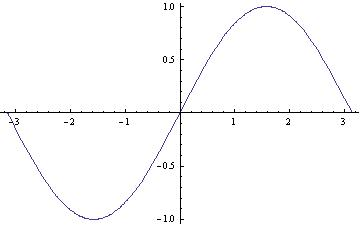
\includegraphics{sin_x.jpg}
% \caption{Transverse momentum distributions}\label{fig:erptsqfit}
% \end{figure}

